% interactcadsample.tex
% v1.03 - April 2017

\documentclass[]{interact}

\usepackage{epstopdf}% To incorporate .eps illustrations using PDFLaTeX, etc.
\usepackage{subfigure}% Support for small, `sub' figures and tables
%\usepackage[nolists,tablesfirst]{endfloat}% To `separate' figures and tables from text if required

\usepackage{natbib}% Citation support using natbib.sty
\bibpunct[, ]{(}{)}{;}{a}{}{,}% Citation support using natbib.sty
\renewcommand\bibfont{\fontsize{10}{12}\selectfont}% Bibliography support using natbib.sty

\theoremstyle{plain}% Theorem-like structures provided by amsthm.sty
\newtheorem{theorem}{Theorem}[section]
\newtheorem{lemma}[theorem]{Lemma}
\newtheorem{corollary}[theorem]{Corollary}
\newtheorem{proposition}[theorem]{Proposition}

\theoremstyle{definition}
\newtheorem{definition}[theorem]{Definition}
\newtheorem{example}[theorem]{Example}

\theoremstyle{remark}
\newtheorem{remark}{Remark}
\newtheorem{notation}{Notation}

% see https://stackoverflow.com/a/47122900


\usepackage{hyperref}
\usepackage[utf8]{inputenc}
\def\tightlist{}
\usepackage[usenames,dvipsnames]{color}
\newcommand{\er}[1]{\textcolor{Plum}{#1}}
\newcommand{\svp}[1]{\textcolor{Green}{#1}}
\newcommand{\rh}[1]{\textcolor{Orange}{#1}}

\begin{document}

\articletype{JSM 2021 Student Paper Competition (ASA sections on Statistical
Computing and Statistical Graphics)}

\title{Perception of exponentially increasing data displayed on a log scale}


\author{\name{Emily A. Robinson$^{a}$, Reka Howard$^{a}$, Susan VanderPlas$^{a}$}
\affil{$^{a}$Department of Statistics, University of Nebraska - Lincoln,}
}

\thanks{CONTACT Emily A. Robinson. Email: \href{mailto:emily.robinson@huskers.unl.edu}{\nolinkurl{emily.robinson@huskers.unl.edu}}, Reka Howard. Email: , Susan VanderPlas. Email: }

\maketitle

\begin{abstract}
Log scales are often used to display data over several orders of
magnitude within one graph. During the COVID-19 pandemic, we have seen
both the benefits and the pitfalls of using log scales to display case
counts, transmission rates, and outbreak regions. In this paper, we
explore the use of linear and log scales to determine whether our
ability to notice differences in the data is different when different
scales are used. Our goal is to provide basic research to support the
principles used to guide design decisions in scientific visualizations
of exponential data. We found that displaying increasing exponential
data on a log scale improved the accuracy of differentiating between
models with slight curvature differences, particularly when identifying
an exponential curve with a lower growth rate than others. When there
was a larger curvature difference, participants accurately
differentiated between the two curves on both the linear and log scale.
An exception occurs when identifying a plot with more curvature than the
surrounding plots, supporting \cite{best_perception_2007} whose results
found that accuracy was higher when nonlinear trends were presented
indicating that it is hard to say something is linear (i.e.~something
has less curvature), but easy to say that it isn't (i.e.~something has
more curvature).
\end{abstract}

\begin{keywords}
Exponential; Log; Visual Inference; Perception
\end{keywords}

\hypertarget{introduction-and-background}{%
\section{Introduction and
Background}\label{introduction-and-background}}

Graphics are a useful tool for displaying and communicating information.
\citep{vanderplas2020testing} Researchers include graphics to
communicate their results in scientific publications and news sources
rely on graphics to convey news stories to the public.
\textcolor{Green}{May want to ask Heather about this one during the meeting (or by email)?}
During the onset of the novel coronavirus pandemic (COVID-19), we saw an
influx of dashboards being developed to display case counts,
transmission rates, and outbreak regions \citep{lisa_charlotte_2020} and
mass media routinely presenting the data on COVID-19
\textcolor{Plum}{\citep{romano_scale_2020}}. People began subscribing to
news sources involved in graphically tracking the coronavirus as a
direct result of these pieces of work and the need for continually
updated information \citep{rost_2020}; thus, gaining more exposure to
the use of graphics. Many of these graphics helped guide decision makers
to implement policies such as shut-downs or mandated mask wearing, but
also facilitated communication with the public to increase compliance
\textcolor{Plum}{\citep{bavel_using_2020}}. With the increasing
importance graphics play in our everyday lives, we must actively choose
which of many possible graphics to draw, according to some set of design
choices to ensure that our charts are effective, as suggested in
\citet{unwin_why_2020}.

When faced with data which spans several orders of magnitude, we must
decide whether to show the data on its original scale (compressing the
smaller magnitudes into relatively little area) or to transform the
scale and alter the contextual appearance of the data. One common
solution is to use a log scale transformation to display data over
several orders of magnitude within one graph. Logarithms make
multiplicative relationships additive, showing elasticities and other
proportional changes, and also linearize power laws
\citep{menge_logarithmic_2018}. When presenting log-scaled data, it is
possible to use either untransformed scale labels (for example, values
of 1, 10 and 100 are equally spaced along the axis) or log-transformed
scale labels (for example, 0, 1, and 2, showing the corresponding powers
of 10). We have recently experienced the benefits and pitfalls of using
log-scales as covid-19 dashboards displayed case count data on both the
log and linear scale
\textcolor{Plum}{\citep{wade_fagen_ulmschneider_2020, financial_times_2020}}.
In spring 2020, during the early stages of the coronavirus pandemic,
there was a large magnitude discrepancy at a given time between
different geographic regions (at all orders of magnitude - states and
provinces as well as countries and continents). During this time, we saw
the usefulness of log-scales showing case count curves for areas with
few cases and areas with many cases within one chart. As the pandemic
evolved, and the case counts were no longer spreading exponentially,
graphs with linear scales seemed more effective at spotting early
increases in case counts that signaled more localized outbreaks. This is
only one recent example of a situation in which both log and linear
scales are useful for showing different aspects of the same data; there
are long histories of using log scales to display results in ecology,
psychophysics, engineering, and physics
\citep{xkcd, menge_logarithmic_2018}.
\textcolor{Green}{XXX it may be interesting to find papers objecting to the use of log scales in some other disciplines beyond ecology.}

Research suggests our perception and mapping of numbers to a number line
is logarithmic at first, but transitions to a linear scale later in
development, with formal mathematics education. This transition to
linear scales occurs first in small numbers (e.g.~1-10) and then
gradually expands to higher orders of magnitude; thus, the logarithmic
intuition about numbers in children is often more noticeable on scales
in the thousands to hundreds of thousands.
\citep{varshney_why_2013, siegler_numerical_2017, dehaeneLogLinearDistinct2008}.
If we percieve logarithmically by default, it is a natural (and
presumably low-effort) way to display information and should be easy to
read and understand/use. In fact, early studies explored the estimation
and prediction of exponential growth, finding that growth is
underestimated when presented both numerically and graphically but that
numerical estimation is more accurate than graphical estimation for
exponential curves. One way to improve estimation of increasing
exponential trends other than changing the scale is through the use of
providing immediate feedback \citep{mackinnon_feedback_1991}. While
prior contextual knowledge or experience with exponential growth does
not improve estimation, previous instruction on exponential growth
reduces the underestimation by adjusting the initial starting value but
not adjusting their perception of growth rate
\citep{wagenaar_misperception_1975, jones_polynomial_1977}. Estimation
was shown to improve when subjects were presented with decreasing
exponential functions \citep{timmers_inverse_1977}.
\citet{jones_polynomial_1977,jones_generalized_1979} and
\citet{wagenaar_extrapolation_1978} propose competing polynomial models
for the perception and extrapolation of exponential series. It seems
that estimation is a two-stage process: first, we identify the type of
curve and direction and then, we use that information for prediction
\citep{best_perception_2007}.

Our inability to accurately predict exponential growth might also be
addressed by log-transforming the data, however, this transformation
introduces new complexities: most readers are not mathematically
sophisticated enough to intuitively understand logarithmic math and
translate that back into real-world effects. In
\citet{menge_logarithmic_2018}, ecologists were surveyed to determine
how often ecologists encounter log-scaled data and how well ecologists
understand log-scaled data when they see it in the literature.
Participants were presented two relationships displayed on linear-linear
scales, log-log scales with untransformed values, or log--log scales
with log-transformed values. \citet{menge_logarithmic_2018} propose
three types of misconceptions participants encountered when presented
data on log-log scales: `hand-hold fallacy', `Zeno's zero fallacy', and
`watch out for curves fallacies'.

In order to provide a set of principles to guide design choices, we must
evaluate these design choices through the use of graphical tests. These
tests may take many forms: identifying differences in graphs, reading
information off of a chart accurately, using data to make correct
real-world decisions, and predicting the next few observations. All of
these types of tests require different levels of use and manipulation of
the information presented in the chart. To lay a foundation for future
exploration of the use of log scales, we begin with the most fundamental
ability to identify differences in charts: this does not require that
participants understand exponential growth, identify log scales, or have
any mathematical training. Instead, we are simply testing the change in
perceptual sensitivity resulting from visualization choices.
\textcolor{Plum}{In \cite{best_perception_2007}, the authors explored whether discrimination between curve types is possible.
They found that accuracy higher when nonlinear trends presented (e.g. it’s hard to say something is linear, but easy to say that it isn’t) and that accuracy is higher with low additive variability.}

A statistic is a numerical function which summarizes the data; by this
definition, graphs are visual statistics. To evaluate a graph, we have
to run our statistic throuugh a visual evaluation - a person. If two
different methods of presenting data result in qualitatively different
results when evaluated visually, then we can conclude that the visual
statistics are significantly different. Recent graphical experiments
have utilized statistical lineups to quantify the perception of
graphical design
choices\citep{vanderplas_clusters_2017, hofmann_graphical_2012, loyVariationsQQPlots2016}.
Statistical lineups provide an elegant way of combining perception and
statistical hypothesis testing using graphical experiments
\citep{wickham2010graphical, majumder_validation_2013, vanderplas_statistical_nodate}.
`Lineups' are named after the `police lineup' of criminal investigations
where witnesses are asked to identify the criminal from a set of
individuals. Similarly, a statistical lineup is a plot consisting of
smaller panels; the viewer is asked to identify the plot of the real
data from among a set of decoy null plots. A statistical lineup
typically consists of 20 panels - 1 target panel and 19 null panels
(Figure \ref{fig:lineup-example}). If the viewer can identify the target
panel embeded within the set of null panels, this suggests that the real
data is visually distinct from data generated under the null model.
Crowd sourcing websites such as Amazon Mechanical Turk, Reddit, and
Proflic allow us to collect responses from multiple viewers. In this
paper, we use statistical lineups to test our ability to differentiate
between increasing exponential data with differing growth rates, using
linear and log scales.

\begin{figure}

{\centering 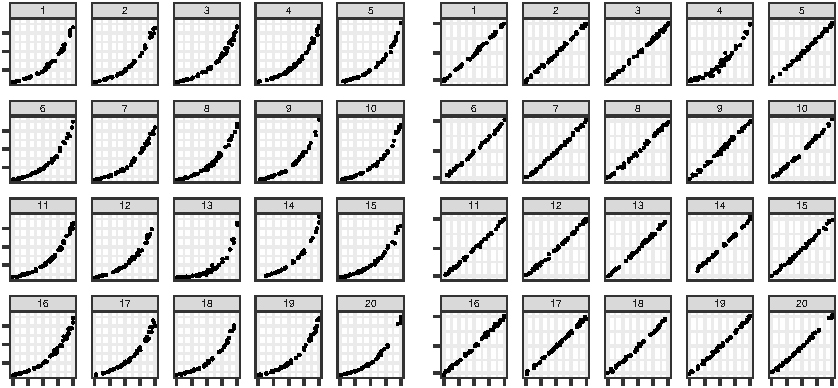
\includegraphics{jsm-2021-student-paper-submission_files/figure-latex/lineup-example-1} 

}

\caption{The plot on the left displays increasing exponential data on a linear scale with panel (2 x 5) + 3 as the target. The plot on the right displays increasing exponential data on the log scale with panel 2 x 2 as the target.}\label{fig:lineup-example}
\end{figure}

\hypertarget{methodology}{%
\section{Methodology}\label{methodology}}

\hypertarget{data-generation}{%
\subsection{Data Generation}\label{data-generation}}

In this study, both the target and null data sets were generated by
simulating data from an exponential model; the models differ in the
parameters selected for the null and target panels. In order to
guarantee the simulated data spans the same range of values, we
implemented a range constraint of \(y\in [10,100]\) and a domain
constraint of \(x\in [0,20]\) with \(N = 50\) points randomly assigned
throughout the domain and mapped to the y-axis using the exponential
model with the selected parameters. These constraints provide some
assurance that participants who select the target plot are doing so
because of their visual perception differentiating between curvature or
slope rather than different starting or ending values.

\textcolor{Plum}{
We simulated data based on a three-parameter exponential model with multiplicative errors: \textcolor{Green}{with parameters defined underneath}
\begin{align}
y_i & = \alpha\cdot e^{\beta\cdot x_i + \epsilon_i} + \theta \\
\text{with } \epsilon_i & \sim N(0, \sigma^2). \nonumber
\end{align} 
}

\noindent The parameters \(\alpha\) and \(\theta\) are adjusted based on
\(\beta\) and \(\sigma^2\) to guarantee the range and domain constraints
are met. The model generated \(N = 50\) points
\((x_i, y_i), i = 1,...,N\) where \(x\) and \(y\) have an increasing
exponential relationship. The heuristic data generation procedure is
provided in Appendix \ref{app:generation}.

The exponential model provides the base for this graphical experiment.
We manipulate the midpoint, \(x_{mid}\), and in turn the estimated
parameters to control the amount of curvature present in the data and
the error standard deviation, \(\sigma\), to control the amount of
deviation from the exponential curve. We selected three midpoints
corresponding to difficulty levels easy (obvious curvature), medium
(noticeable curvature), and hard (almost linear) along with a sensible
choice of standard deviation, \(\sigma\). The midpoints and standard
deviation combinations were chosen using a method described in
\cite{vanderplas_clusters_2017}; additional details and final parameter
values are available in Appendix \ref{app:parameters}.

\hypertarget{lineup-setup}{%
\subsection{Lineup Setup}\label{lineup-setup}}

The lineup plots were generated by mapping simulating data corresponding
to difficulty level A to a scatterplot while the null plots were
generated by mapping simulated data corresponding to difficulty level B
to a scatterplot. For example, a target plot with simulated data
following an increasing exponential curve with obvious curvature is
embeded within null plots with simulated data following an increasing
exponential that is almost linear (i.e.~Easy-Hard). By our constraints,
the target plot and null plots will span a similar domain and range.
There are a total of 6 (i.e.~3 choose 2) lineup parameter combinations.
Two sets of each lineup parameter combination were simulated (total of
12 test datasets) and plotted on both the linear and the log scale
(total of 24 test lineup plots). In addition, there are three parameter
combinations which generate homogeneous ``Rorschach'' lineups, where all
panels are from the same distribution. Each participant evaluated one of
these lineups, but for simplicity, these evaluations are not described
in this paper.

\hypertarget{study-design}{%
\subsection{Study Design}\label{study-design}}

Each participant was shown a total of thirteen lineup plots (twelve test
lineup plots and one Rorschach lineup plot). Participants were randomly
assigned one of the two replicate datasets for each of the six unique
lineup parameter combinations. For each assigned test dataset, the
participant was shown the lineup plot corresponding to both the linear
scale and the log scale. For the additional Rorschach lineup plot,
participants were randomly assigned a one data set shown on either the
linear or the log scale. The order of the thirteen lineup plots shown
was randomized for each participant.

Participants above the age of majority were recruited from Reddit's
Visualization and Sample Size communities. Since participants recruited
on Reddit were not compensated for their time, most participants have an
interest in data visualization research. Previous literature suggests
that prior mathematical knowledge or experience with exponential data is
not associated with the outcome of graphical experiments
\citep{vanderplasSpatialReasoningData2016}. Participants completed the
experiment using a Shiny applet
(\url{https://shiny.srvanderplas.com/log-study/}).

Participants were shown a series of lineup plots and asked to identify
the plot that was most different from the others. On each plot,
participants were asked to justify their choice and provide their level
of confidence in their choice. The goal of this experimental task is to
test an individuals ability to perceptually differentiate exponentially
increasing data with differing rates of change on both the linear and
log scale.

\hypertarget{results}{%
\section{Results}\label{results}}

Participant recruitment through Reddit occurred over the course of two
weeks during which 58 individuals completed 518 unique test lineup
evaluations. Participants who completed fewer than 6 lineup evaluations
were removed from the study (17 participants, 41 evaluations). The final
dataset included a total of 41 participants and 477 lineup evaluations.
Each plot was evaluated by between 18 and 28 individuals (Mean: 21.77,
SD: 2.29). In 67\% of the 477 lineup evaluations, participants correctly
identified the target panel.

Target plot identification was analyzed using the Glimmix Procedure in
SAS 9.4. Each lineup plot evaluated was assigned a value based on the
participant response (correct = 1, not correct = 0). The binary response
was analyzed using generalized linear mixed model following a binomial
distribution with a logit link function following a row-column blocking
design accounting for the variation due to participant and data set
respectively, with a split plot design accounting for the same
participant evaluating the same dataset on both the linear scale and log
scale. See target plot identification model details and estimates in
Appendix \ref{app:glmm-model}

On both the log and linear scales, the highest accuracy occured in
lineup plots where the target model and null model had large curvature
differences (e.g.~easy-hard and hard-easy). When comparing models that
have slight curvature differences (e.g.~Medium-Easy), there is a
sacrifice in accuracy when displayed on the linear scale. It is worth
noting that there is a more significant decrease in accuracy on the
linear scale when comparing a target plot with a lower rate of change
embedded in null plots with higher rates of change (e.g.~Medium-Easy and
Hard-Medium). This agrees with \cite{best_perception_2007} whose results
found that accuracy was higher when nonlinear trends were presented
indicating that it is hard to say something is linear (i.e.~something
has less curvature), but easy to say that it isn't (i.e.~something has
more curvature). Overall, there is are no significant differences in
accuracy between curvature combinations when data is presented on a log
scale indicating participants were consistent in their success of
identifying the target panel on the log scale.
\textcolor{Plum}{Figure \ref{fig:odds-ratio-plot} displays the estimated (log) odds ratio of successfully identifying the target panel on the log scale compared to the linear scale. We found the choice of scale has no impact if curvature differences are large. However, presenting data on the log scale makes us more sensitive to the the changes when there are only slight changes in curvature.}

\begin{figure}

{\centering 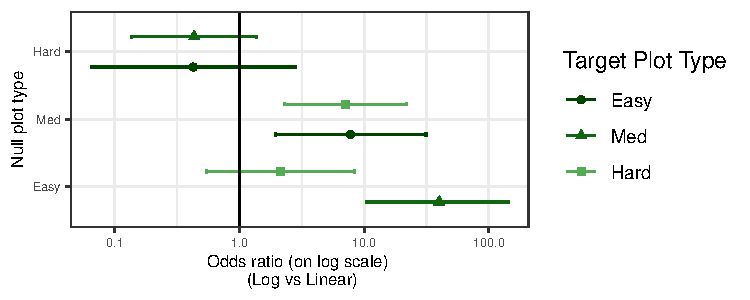
\includegraphics{jsm-2021-student-paper-submission_files/figure-latex/odds-ratio-plot-1} 

}

\caption{Odds Ratio's}\label{fig:odds-ratio-plot}
\end{figure}

\hypertarget{discussion-and-conclusion}{%
\section{Discussion and Conclusion}\label{discussion-and-conclusion}}

The overall goal of this paper is to provide basic research to support
the principles used to guide design decisions in scientific
visualizations of exponential data. In this study, we explored the use
of linear and log scales to determine whether our ability to notice
differences in the data is different when different scales are used.
\textcolor{Plum}{Our results indicated that displaying increasing exponential data on a log scale improved the accuracy of differentiating between models with slight curvature differences, particularly when identifying an exponential curve with a lower growth rate than others. 
When there was a larger curvature difference, participants accurately differentiated between the two curves on both the linear and log scale. An exception occurs when identifying a plot with more curvature than the surrounding plots, supporting \cite{best_perception_2007} whose results found that accuracy was higher when nonlinear trends were presented indicating that it is hard to say something is linear (i.e. something has less curvature), but easy to say that it isn't (i.e. something has more curvature).}

Further experimentation is necessary to test an individual's ability to
make predictions for exponentially increasing data. Previous literature
suggests that we tend to underestimate predictions of exponentially
increasing
data.\citep{jones_generalized_1979, jones_polynomial_1977, wagenaar_extrapolation_1978}.
\citep{mosteller_eye_1981} designed and carried out an empirical
investigation to explore properties of lines fitted by eye. The
researchers found that students tended to fit the slope of the first
principal component or major axis (the line that minimizes the sum of
squares of perpendicular rather than vertical distances) and that
students who gave steep slopes for one data set also tended to give
steep slopes on the others. Interestingly, the individual-to-individual
variability in slope and in intercept was near the standard error
provided by least squares. A similar graphical task is used in the New
York Times ``You Draw It'' page asking readers to test their knowledge
by using their curser to estimate values of a certain topic under
different political administrations or over different years
\textcolor{Plum}{(CITE THIS)}. In addition to differentiation and
prediction of exponentially increasing data, it is of interest to test
an individuals ability to translate a graph of exponentially increasing
data into real value quantities and extend their estimations by making
comparisons. \citep{friel_making_2001} emphasize the importance of graph
comprehension proposing that the graph construction plays a role in the
ability to read and interpret graphs.

\hypertarget{supplementary-materials}{%
\section*{Supplementary Materials}\label{supplementary-materials}}
\addcontentsline{toc}{section}{Supplementary Materials}

\begin{itemize}
\item
  \textbf{Appendix:}
\item
  \textbf{Code:} R code to reproduce figures of the article as well as
  SAS code to fit models used in the article.
  (\href{https://github.com/srvanderplas/Perception-of-Log-Scales/blob/master/manuscripts/jsm-2021-student-paper-submission/code/image-generator.R}{image-generator.R},
  R file;
  \href{https://github.com/srvanderplas/Perception-of-Log-Scales/blob/master/lineups-pilot-analysis/sasCode/glmm-analysis-jsm-student-paper.sas}{glmm-analysis-jsm-student-paper.sas},
  SAS file)
\item
  \textbf{Data:} Anonymized responses from the Reddit study to
  investigate the use of logarithmic scales. Each line corresponds to
  one lineup evaluation by a participant.
  (\href{https://github.com/srvanderplas/Perception-of-Log-Scales/blob/master/lineups-pilot-analysis/data/jsm-student-paper-11302020.csv}{jsm-student-paper.csv},
  csv file)
\end{itemize}

\clearpage
\appendix

\hypertarget{data-generation-procedure}{%
\section{\texorpdfstring{Data Generation
Procedure\label{app:generation}}{Data Generation Procedure}}\label{data-generation-procedure}}

\textit{Algorithm 2.1.1: Paremeter Estimation}

Input Parameters: domain \(x\in[0,20]\), range \(y\in[10,100]\),
midpoint \(x_{mid}\).

Output: estimated model parameters \(\hat\alpha, \hat\beta, \hat\theta\)

\begin{enumerate}
\def\labelenumi{\arabic{enumi}.}
\item
  Determine the \(y=-x\) line scaled to fit the assigned domain and
  range.
\item
  Map the values \(x_{mid} - 0.1\) and \(x_{mid} + 0.1\) to the \(y=-x\)
  line for two additional points.
\item
  From the set points \((x_k, y_k)\) for \(k = 1,2,3,4\), obtain the
  coefficients from the linear model \(\ln(y_k) = b_0 +b_1x_k\) to
  obtain starting values -
  \(\alpha_0 = e^{b_0}, \beta_0 = b_1, \theta_0 = 0.5\cdot \min(y)\)
\item
  Using the \texttt{nls()} function from the \texttt{stats} package in
  Rstudio and the starting parameter values -
  \(\alpha_0, \beta_0, \theta_0\) - fit the nonlinear model,
  \(y_k = \alpha\cdot e^{\beta\cdot x_k}+\theta\) to obtain estimated
  parameter values - \(\hat\alpha, \hat\beta, \hat\theta.\)
\end{enumerate}

\noindent\textit{Algorithm 2.1.2: Exponential Simulation}

Input Paremeters: sample size \(N = 50\), estimated parameters
\(\hat\alpha\), \(\hat\beta\), and \(\hat\theta\), \(\sigma\) standard
\indent deviation from the exponential curve.

Output Parameters: \(N\) points, in the form of vectors \(\mathbf{x}\)
and \(\mathbf{y}\).

\begin{enumerate}
\def\labelenumi{\arabic{enumi}.}
\item
  Generate \(\tilde x_j, j = 1,..., N\cdot \frac{3}{4}\) as a sequence
  of evenly spaced points in \([0,20]\). This ensures the full domain of
  \(x\) is used, fulfilling the constraints of spanning the same domain
  and range for each parameter combination.
\item
  Obtain \(\tilde x_i, i = 1,...N\) by sampling \(N = 50\) values from
  the set of \(\tilde x_j\) values. This gaurantees some variability and
  potential clustring in the exponential growth curve disrupting the
  perception due to continuity of points.
\item
  Obtain the final \(x_i\) values by jittering \(\tilde x_i\).
\item
  Calculate \(\tilde\alpha = \frac{\hat\alpha}{e^{\sigma^2/2}}.\) This
  ensures that the range of simulated values for different standard
  devaition parameters has an equal expected value for a given rate of
  change due to the non-constant variance across the domain.
\item
  Generate
  \(y_i = \tilde\alpha\cdot e^{\hat\beta x_i + e_i}+\hat\theta\) where
  \(e_i\sim N(0,\sigma^2).\)
\end{enumerate}

\hypertarget{parameter-selection}{%
\section{\texorpdfstring{Parameter Selection
\label{app:parameters}}{Parameter Selection }}\label{parameter-selection}}

For each level of difficulty, we simulated 1000 data sets of
\((x_{ij}, y_{ij})\) points for \(i = 1,...,50\) and \(j = 1...10\).
Each generated \(x_i\) point from \textit{Algorithm 2.1.2} was
replicated 10 times.Then the lack of fit statistic (LOF) was computed
for each simulated dataset by calculating the deviation of the data from
a linear line. Plotting the density curves of the LOF statistics for
each level of difficulty choice allows us to evaluate the ability of
differentiating between the difficulty levels and thus detecting the
target plot. In Figure \ref{fig:lof-density-curves}, we can see the
densities of each of the three difficulty levels. While the LOF
statistic provides us a numerical value for discriminating between the
difficulty levels, we cannot directly relate this to the perceptual
discriminability; it serves primarily as an approximation to ensure that
we are testing parameters at several distinct levels of difficulty.

\begin{figure}

{\centering 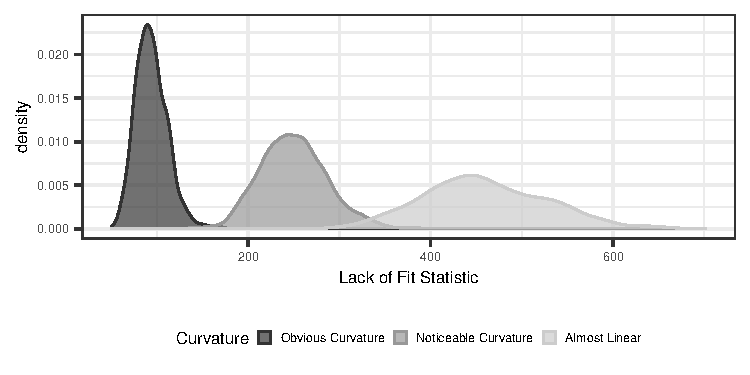
\includegraphics{jsm-2021-student-paper-submission_files/figure-latex/lof-density-curves-1} 

}

\caption{Density plot of the lack of fit statistic showing separation of difficulty levels: obvious curvature, noticable curvature, and almost linear.}\label{fig:lof-density-curves}
\end{figure}

Final parameter estimates are shown in Table \ref{tab:parameter-data}.

\begin{table}

\caption{\label{tab:parameter-data}Final parameters used to simulate exponential data for each of the three diffculty levels: Easy (Obvious curvature), Medium (noticable curvature) and Hard (almost linear)}
\centering
\begin{tabular}[t]{ccccccc}
\toprule
 & $x_{mid}$ & $\hat\alpha$ & $\tilde\alpha$ & $\hat\beta$ & $\hat\theta$ & $\hat\sigma$\\
\midrule
Easy & 14.5 & 0.91 & 0.88 & 0.23 & 9.10 & 0.25\\
Medium & 13.0 & 6.86 & 6.82 & 0.13 & 3.14 & 0.12\\
Hard & 11.5 & 37.26 & 37.22 & 0.06 & -27.26 & 0.05\\
\bottomrule
\end{tabular}
\end{table}

\hypertarget{target-plot-identification-model-details}{%
\section{\texorpdfstring{Target Plot Identification Model Details
\label{app:glmm-model}}{Target Plot Identification Model Details }}\label{target-plot-identification-model-details}}

\textcolor{Plum}{
Target plot identification was analyzed using the Glimmix Procedure in SAS 9.4. 
Each lineup plot evaluated was assigned a value based on the participant response (correct = 1, not correct = 0). 
Define $Y_{ijkl}$ to be the event that participant $l$ correctly identifies the target plot for dataset $k$ with curvature $j$ plotted on scale $i$. 
The binary response was analyzed using generalized linear mixed model following a binomial distribution with a logit link function following a row-column blocking design accounting for the variation due to participant and data set respectively, with a split plot design accounting for the same participant evaluating the same dataset on both the linear scale and log scale as shown in the Equation (2).
\begin{equation}
\text{logit }P(Y_{ijk}) = \eta + \delta_i + \gamma_j + \delta \gamma_{ij} + s_l + d_k + wp_{jkl}
\end{equation}
where
\begin{align*}
&\eta               \text{ is the beaseline average probability of selecting the target plot.} \\
&\delta_i           \text{ is the effect of the log/linear scale.} \\
&\gamma_j           \text{ is the effect of the curvature combination.} \\
&\delta\gamma_{ij}  \text{ is the two-way interaction effect of the scale and curvature.} \\
&s_l \sim N(0,\sigma^2_\text{{participant}}), \text{ random effect for participant characteristics} \\
&d_k \sim N(0,\sigma^2_{\text{dataset}}), \text{ random effect for data specific characteristics.} \\
&wp_{jkl} \sim N(0,\sigma^2_\text{{whole-plot}}), \text{ random effect for the particular participant by dataset charactersitics.}
\end{align*}
We assume that random effects for dataset, participant, and whole plot effects are independent. See least squares means estimated probabilities and Tukey groupings at an $\alpha = 0.05$ significance level in Figure \ref{fig:lsmeans-plot}.
}

\textcolor{Plum}{Add details here: ANOVA, p-values, pairwise comparisons, etc.}

\begin{figure}

{\centering 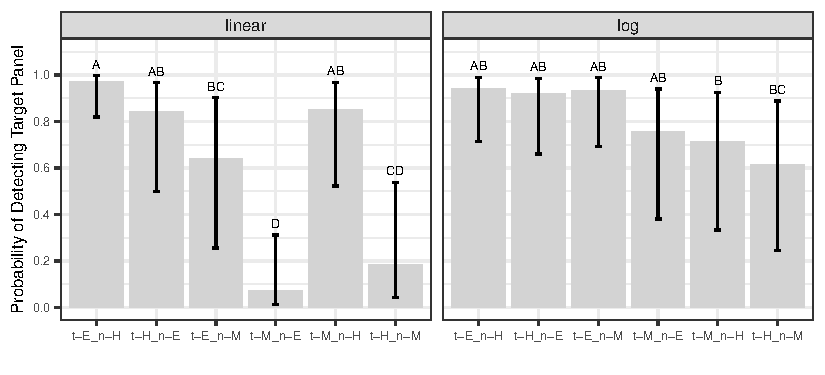
\includegraphics{jsm-2021-student-paper-submission_files/figure-latex/lsmeans-plot-1} 

}

\caption{Least Squares Means}\label{fig:lsmeans-plot}
\end{figure}

\bibliographystyle{tfcad}
\bibliography{references.bib}




\end{document}
